\chapter{Literature review}\label{sec:review}
In this chapter, previous work on the optimisation of network tied-arch bridges is summarised. After the first bridges of this type were built in the 1960s, the hanger inclination drew the focus of the researchers. 
It governs the structural behaviour with respect to many aspects, of which mainly hanger unloading was investigated. Only in the last two decades, with the rise of its popularity, researchers also considered its other individual aspects. However, no broad discussion evolved on most of them. 
In most studies, single aspects are investigated, such as hanger unloading or the hanger forces in general, fatigue or cable loss.
These aspects, which have been investigated in parametric studies, are introduced in \cref{sec:rev_forces} to \cref{sec:rev_loss}. Besides parametric studies, numerical optimisation methods have been used to identify the tendencies and further optimise multiple parameters simultaneously. Recently, these methods have been used to minimise the weight of network tied-arch bridges or the costs of other bridge structures. The respective approaches are introduced in \cref{sec:rev_weight} and \cref{sec:rev_cost}. 
Few authors introduced design methodologies to allow for a fast and approximately optimised initial design. These methods are presented and critically evaluated in \cref{sec:rev_meth}. Further, a previous Master Thesis, which builds the foundation of this Thesis, is summarised in \cref{sec:rev_prev}. Besides the hanger arrangement it addresses the arch shape and the self-equilibrium stress state. Ultimately, this chapter is summarised in \cref{sec:rev_sum}.

\section{Hanger forces} \label{sec:rev_forces}
Per Tveit, described the concept of network tied-arch bridges in his dissertation in 1959 and designed two of the first bridges of this type in 1963 in Norway.
He investigated the parallel hanger net and the constant change of inclination arrangement, aiming to prevent hanger unloading, which is a critical issue under asymmetric loading for short-span bridges \cite{Tveit_66}.
It was found that, whereas flat inclinations are more suitable to prevent hanger unloading, they also result in higher hanger forces. To find a solution for these opposing objectives, he developed diagrams, which predict the maximum hanger inclination without hanger unloading depending on the ratio of life to dead loads. As a first optimisation of the hanger arrangement, he proposed increasing the hangers' inclinations as much as possible before the first hanger unloading occurs. Later, he additionally recommended constant hanger spacing on the arch with one hanger per node to minimise the resulting bending moments.  \medskip

In 2012, Teich conducted an extensive parameter study varying the key in-plane parameters to investigate the hanger force-related objectives \cite{Teich}. Namely, these objectives are the maximum force, its variation, the cyclic stresses and the number of unloaded cables.% without considering the three hangers closest to the knuckle. 
The parameters such as span, rise, number of hangers and their arrangement are varied in the study, leading to approximately \SI{90000}{} variants. The only in-plane parameter which is left constant is the circular arch shape. The cross sections of the arch rib and the tie girder were obtained in a simplified preliminary design assuming a steel carriageway. Each variant was then analysed in a two-dimensional model under unilateral and full vertical train live loading. 
Again, hanger unloading posed a big issue for many variants and affected all investigated objectives. Therefore, Teich recommends the arrangement of 36 to 52 hangers per plane for spans between \SI{100}{m} and \SI{250}{m}. Further, he recommends flat inclinations between $50\degree$ and $55\degree$ for the parallel hanger pattern to solve the hanger unloading problem. The constant change of inclination arrangement offers significant advantages and relies on large changes in inclination. However, the radial arrangement with an intersection angle $\beta=36\degree$ was found the best regarding virtually all the considered objectives. Based on the normalised addition of the objectives, Teich also developed a design methodology, which is explained in Section \ref{sec:rev_meth}. 
It has to be noted that both Tveit and Teich did not consider prestressing of the hangers in their models. It is implicitly assumed that the permanent hanger forces correspond to the elastic response under permanent loads. Also, the ratio of live to dead loads is assumed to be exceptionally high (up to $p/g=1$). Therefore, the impact of hanger unloading is significantly overestimated compared to common network tied-arch bridges featuring a concrete deck.

\section{Fatigue} \label{sec:rev_fat}
Pellegrino et al. evaluated hanger patterns with respect to fatigue on a bridge featuring a composite deck with a life to dead load ratio of $p/g=0.3$ and a span of \SI{100}{m} \cite{Pellegrino}. The considered hanger patterns are the constant change of inclination and the radial arrangement, which are also compared to a vertical arrangement. It is found that vertical hangers are advantageous over network arrangements concerning the maximum and average cyclic stresses. By inclining the vertical hangers, the behaviour deteriorates strongly and improves again for flat inclinations. Especially the flat hangers of the radial arrangement near the knuckle undergo very high cyclic stresses, and various modifications to reduce the maximum cyclic stress are studied. However, no generally applicable modification independent of the intersection angle was found. Therefore, it is recommended to design the hangers near the knuckle independent of the hanger arrangement pattern. Steeper hangers near the knuckles are generally good advice to start with. For a radial hanger arrangement with 22 hangers per set, it is recommended to arrange the last five hangers of each set parallel to the previous one, as shown in \autoref{fig:Pellegrino}.
\begin{figure}[H]
    \centering
    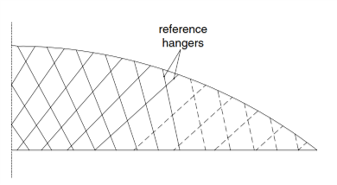
\includegraphics[trim={0 0.6cm 0 0.4cm},clip, width=0.55\textwidth]{Pictures/PellegrinoArrangement.png}
    \caption{Modified radial arrangement (adopted from \cite{Pellegrino})}
    \label{fig:Pellegrino}
\end{figure}


\section{Cable loss} \label{sec:rev_loss}

Most of the work dedicated to cable loss focuses on cable-stayed bridges, for which it is not unusual, that this accidental limit state governs the design of the superstructure. Wolff and Starossek pointed out that the loss of two or more cables can even impair the global stability of a cable-stayed bridge \cite{Wolff}. In an investigation on the Blennerhassett Island Bridge, Zoli and Woodward showed that a network tied-arch bridge offers more redundancy and can even withstand the loss of multiple cables \cite{Zoli}. However, it is concluded that cable loss should be a key consideration for network tied-arch bridges' design process. Further, it is concluded that a detailed dynamic analysis can allow for a significant reduction of the dynamic amplification factor due to cable loss.

Bruno et al. conducted a study on the behaviour of network tied-arch bridges to identify the critical factors on the effects under cable loss \cite{Bruno}. The behaviour is studied using the simplified quasi-static approaches of the PTI and the Eurocode compared to a dynamic non-linear FE-analysis \cite{PTI}. As a reference case, a bridge with a span of \SI{180}{m} and a rise of \SI{30}{m} is studied featuring a parallel hanger arrangement with 17 hangers per set and an inclination of $65 \degree$. Further, prestressing is taken into account using the zero-displacement method. It was found, that the most dangerous cables to lose are the ones located near the quarter points of the tie and are inclined towards the crown of the arch. The corresponding vertical displacements are maximal for this hanger with a value of $L/4000$. The stresses in the neighbouring hangers of the same set increase by 60\% through the loss of the cable at the quarter-point. The other set's hangers are less affected increasing by a maximum of less than 25\%, as shown in \cref{fig:Bruno}. It is concluded, that also the simplified method by the PTI provides an adequate degree of accuracy, as it only underestimates the hanger forces in the less affected hanger set.
\begin{figure}[H]
    \centering
    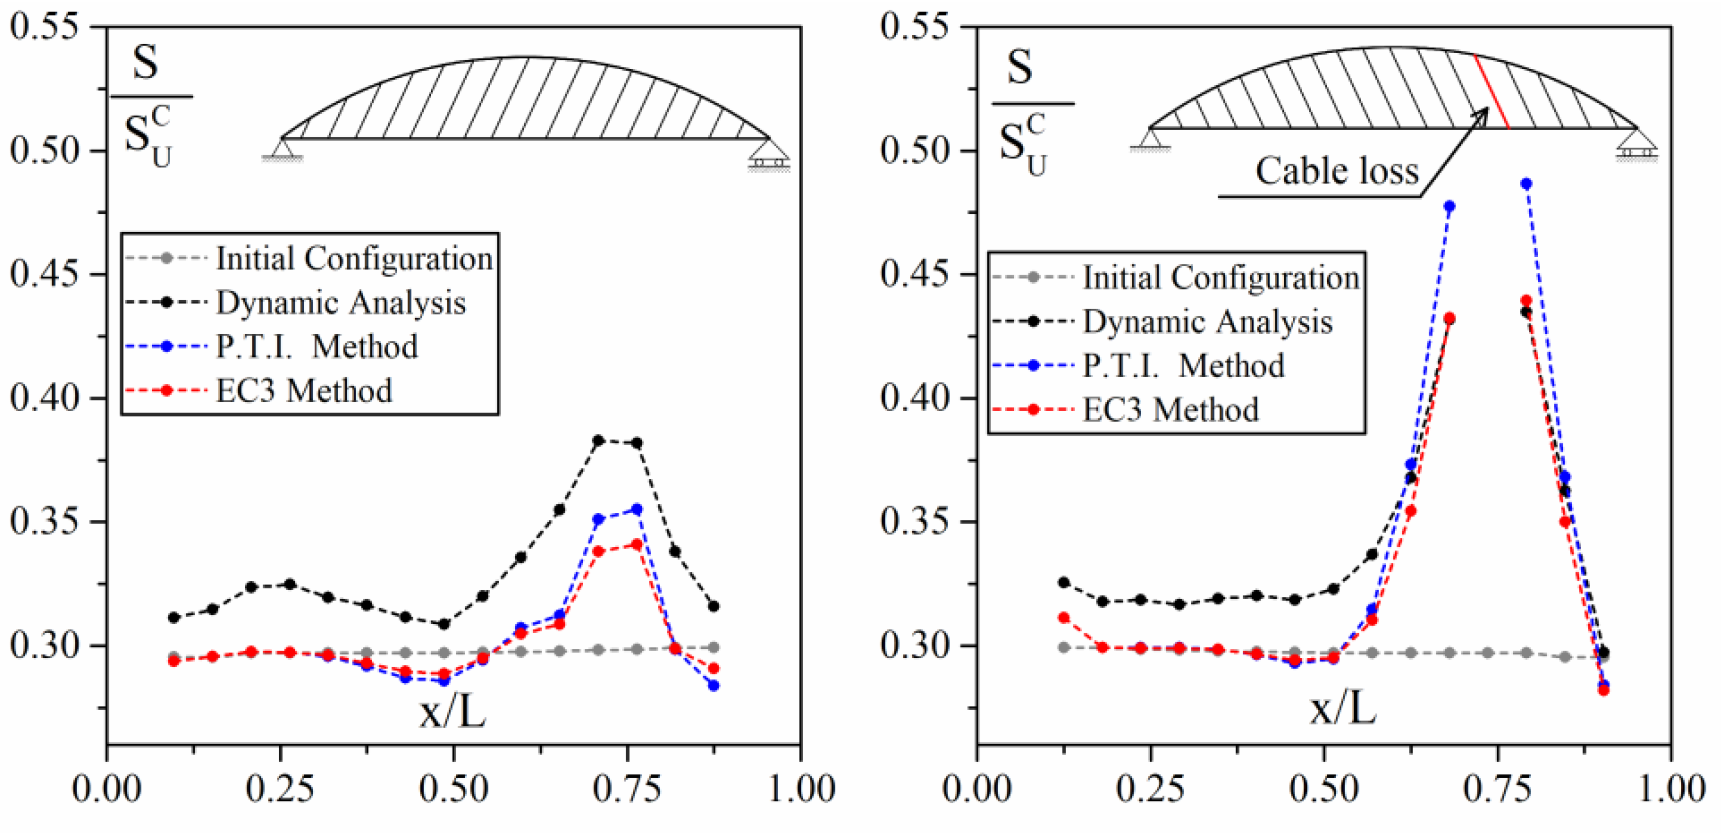
\includegraphics[width=0.65\textwidth]{Pictures/BrunoCableLoss.PNG}
    \caption{Stress distribution in the hanger sets (adopted from \cite{Bruno})}
    \label{fig:Bruno}
\end{figure}

Further, it was found that parallel arrangements with flatter inclinations cause the displacements and the internal forces to increase. Restricted to the plausible range of $50\degree$ to $70\degree$, differences in the deflections amounting up to 20\% can be expected. In \cref{fig:Bruno2}, the respective displacements are also compared to the arrangement with vertical hangers, specifying the hangers' total volumes. It is seen that the vertical arrangement performs significantly better despite using a smaller quantity of cable material. Compared to hanger forces and fatigue investigations, an opposite tendency is observed, where the behaviour improves for steeper hangers. This advantage is attributed to the stiffer behaviour of the respective structure.
\begin{figure}[H]
    \centering
    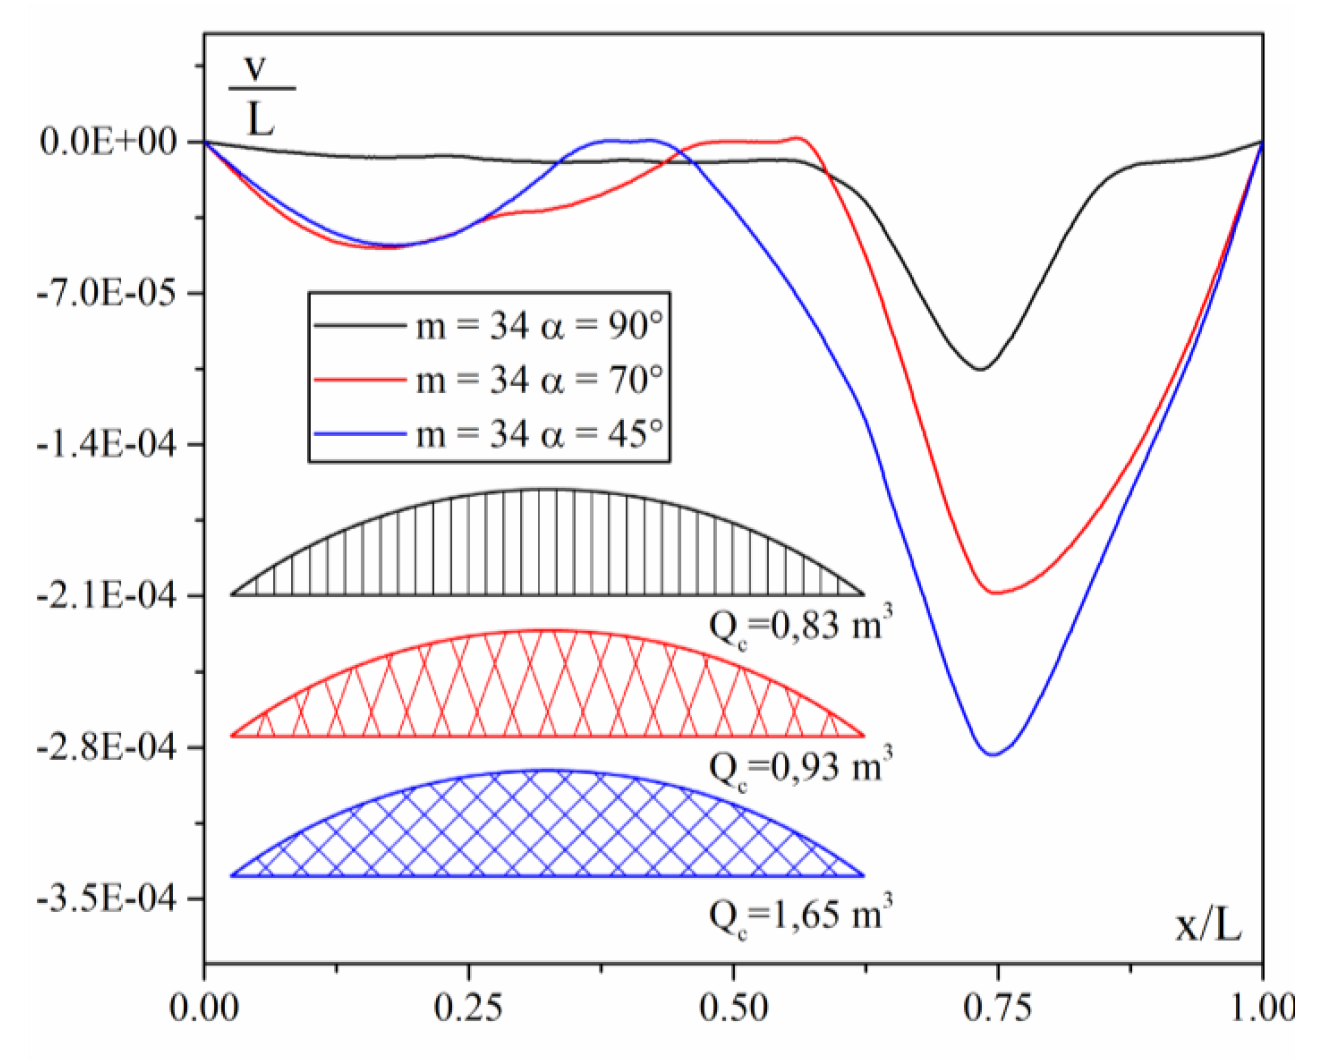
\includegraphics[width=0.50\textwidth]{Pictures/BrunoArrangements.PNG}
    \caption{Vertical deflections under cable loss (adopted from \cite{Bruno})}
    \label{fig:Bruno2}
\end{figure}

\section{Structural weight} \label{sec:rev_weight}
In other applications of structural optimisation methods, such as additive manufacturing, the structure's weight is an established and efficient objective function \cite{Plocher}.
Also in civil engineering, researchers have recently used numerical optimisation methods over parametric studies and partially adopted the minimum weight formulation \cite{MARTINS}.
Technically, all parameters describing a network tied-arch bridge's design can be considered, given enough computational resources. 
However, as it is usually not intended to optimise a full design, it is still preferred to limit the process to a few key variables. 
Belevicius et al. optimised a pedestrian network tied-arch bridge with respect to the weight for different boundary conditions and using nine design variable \cite{Belevicius}. 
As some of the parameters are discrete, the problem is mathematically described as a constrained mixed-integer problem. It is solved using a genetic algorithm with penalisation for the design conditions.
Even with the relatively limited number of parameters, the optimised designs are well dispersed over the feasible domain, accentuating the underlying problem's multi-modality.
Even after reducing the number of parameters, the results do not resemble typical tied-arch bridges, be it for the high amount of hangers or the large rise-to-span ratios. 
Ultimately, a strongly varying hanger pattern is recommended, and a rise-to-span ratio of up to 0.23.
Therefore, the aim of finding a fast and straightforward method for obtaining the full initial design is reached only in an unsatisfactory manner as it gives somewhat random results.
It demonstrates well the difficulties associated with numerical optimisation for design purposes. 
It is likely, that an oversimplified objective function, considering only the weights, yielded these odd designs. 
The unfactored weights neglect the differences in the unit costs of the different components, favouring the arrangement of additional hangers in particular.


\section{Structural costs} \label{sec:rev_cost}
Design optimisations often take the goal of minimising the structural costs as an objective. Recently, researchers have used a wide range of optimisation methods to solve problems with geometrical, topological and mechanical design variables underlying different sets of structural constraints \cite{MARTINS}. However, the field's main focus lies again on cable-stayed bridges, and further, only a single publication attempted to take the construction expenses into the objective. It is critical to remember, that for the slender network tied-arch bridges a high ratio of the costs is made up by labour and not by the material and the fabrication of the components \cite{Tveit_How}. Therefore, the estimated structural costs can serve well as a guideline. However, it makes sense, to keep the focus on the structural considerations.

\section{Design methodologies} \label{sec:rev_meth}
The complex behaviour and the wide range of associated challenges of the network tied-arch bridge are partially responsible for its comparably sparse use \cite{Tveit_How}. Design guidelines or design methodologies are essential to promote this bridge type's construction, as an engineer cannot conduct a full investigation. However, only a few authors have addressed this challenge for network tied-arch bridges.
Teich developed a design methodology based on the results of an extensive parameter study \cite{Teich}. He transformed the four hanger-related objectives into a normalised score and added them to rank the investigated designs. In the first step of the methodology, the number of hangers is chosen according to the recommended values depending on the bridge's span, as shown in \cref{tab:Teich_hangers}. Using the number of hangers and the span, the optimal hanger arrangement pattern is chosen using a different table, in which the arrangements are ranked according to their normalised score. For all cases, either the constant change of inclination or the radial arrangement is the recommended choice. Ultimately, the best set of parameters can be chosen depending on the number of hangers in a table corresponding to the respective hanger set. An example of the constant change of inclination arrangement is shown in \cref{tab:Teich_hangers_2}, adapted to the parameters used in this Thesis. Further, it is recommended to arrange the three hangers closest to the knuckle independent of the pattern.

\begin{table}[H]
\centering
\caption{Recommended number of hangers (adopted from \cite{Teich})}
\label{tab:Teich_hangers}
\begin{tabular}{lccccc}
\toprule
Span & $< \SI{100}{m}$ & \SI{100}{m} & \SI{150}{m} & \SI{200}{m} & \SI{250}{m} \\ \midrule
Number of hangers & 30-44 & 36-46 & 38-48 & 40-50 & 42-52 \\ \bottomrule
\end{tabular}
\end{table}

\begin{table}[H]
\centering
\caption{Recommended parameters for the constant change arrangement (adopted from \cite{Teich})}
\label{tab:Teich_hangers_2}
\begin{tabular}{lcccccccc}
\toprule
Span & \multicolumn{4}{|c|}{$<\SI{150}{m}$} & \multicolumn{4}{c}{$> \SI{150}{m}$} \\
Number of hangers & \multicolumn{1}{|c}{24} & 36 & 48 & \multicolumn{1}{c|}{60} & 24 & 36 & 48 & 60 \\ \midrule
Maximum inclination & 75\degree & 82\degree & 85\degree & 83\degree & 75\degree & 87\degree & 90\degree & 90\degree \\
Average inclination & 57\degree & 56\degree & 52\degree & 49\degree & 57\degree & 61\degree & 55\degree & 53\degree \\ \bottomrule
\end{tabular}
\end{table}

Whereas this methodology is relatively simple to use, it lacks a specific boundary of the application. For most network tied-arch bridges it significantly overestimates the number of hangers. For the Blennerhassett Island Bridge's span, between 42 and 52 hangers are recommended compared to the 26 hangers that were designed. This overestimation is partially due to the live load, which almost equals the dead load in the analysis underlying the methodology. Further, only normal forces were considered for judging the optimality of the structure. This is a significant oversimplification of the actual objective of an optimised design. The claimed generality of these design guidelines, therefore has to be questioned.\medskip

Bruno points out that most design guidelines do not give advice on the permanent bridge configuration and neither yield an optimised design with respect to material use. Therefore, he introduced a three-step design methodology overcoming the numerical challenges of the often-used metaheuristic optimisation methods \cite{Bruno}. Starting with an initial design, the zero-configuration is determined by a method similar to the zero-displacement method. 
It yields the individual prestressing forces for each hanger. In a second step, the structure is analysed under the action of live loads. If the design conditions are not verified, the hanger cross sections are individually are adapted. The arch rib and the tie girder can followingly be designed on the obtained distributions of internal forces. This procedure is repeated iteratively until the changes lie within a certain tolerance. It efficiently yields a solution with the lowest possible material utilisation and the corresponding initial configuration. 
However, for most engineers, this design procedure exceeds their knowledge and practice in numerical optimisation. Further, the assignment of different cross sections for each hanger is usually disregarded for unambiguity. While this methodology overcomes the computational effort and convergence problems of pure optimisation methods, it lacks the simplicity to be a suitable tool for a designer.

\section{Arch shape} \label{sec:rev_prev}
In a previous Master's Thesis at the Chair of Structural Engineering for Concrete Structures and Bridge Design, Riccardo Cavegn investigated the optimal arch shape \cite{Cavegn}. The investigation is based on an optimised self-equilibrium stress state, and the obtained designs were ultimately compared by their estimated costs. The arch shape's dependency on the hanger arrangement was studied in particular, with the Blennerhassett Island Bridge as a reference. The constant change of inclination arrangement and its subset, the parallel arrangement, were considered in the optimisation and analysed in a comparative parametric study. 
In the first step, the hangers' prestressing was determined to minimise the bending moments under dead loads. To achieve this, the hanger tuning matrix relating the individual unit strains of the hangers to the bending moments along the tie girder was calculated using structural analysis software. This matrix was then used to determine the prestrains giving minimal bending moments in the tie girder, as shown in \cref{fig:Cavegn3}. In a second step, the obtained hanger forces were used to graphically construct the arch's thrust line as illustrated in \autoref{fig:Cavegn4}. As the two steps influence each other, they are repeated iteratively until the obtained arch geometry stabilises.
\begin{figure}[H]
\centering
\begin{subfigure}{0.5\textwidth}
    \centering
    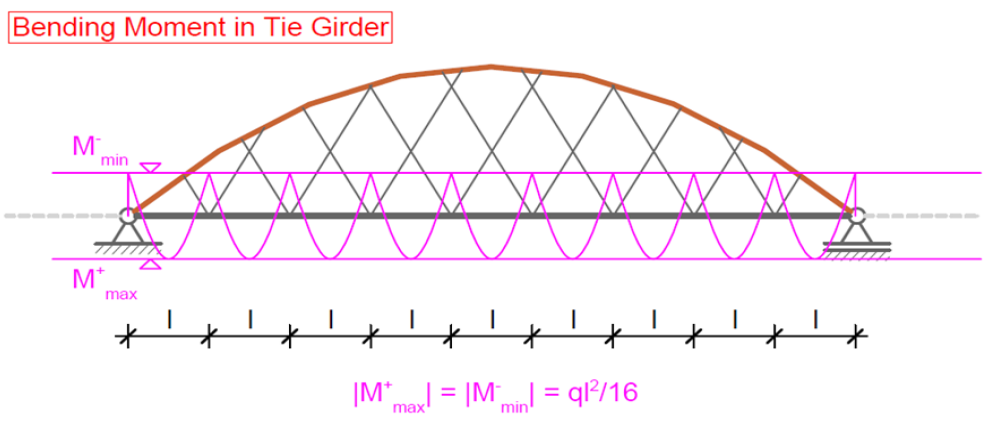
\includegraphics[width=0.73\textwidth]{Pictures/OptimizedBendingMoment.PNG}
    \caption{Determination of the self-equilibrium stress state}
    \label{fig:Cavegn3}
\end{subfigure}%
\begin{subfigure}{.5\textwidth}
    \centering
    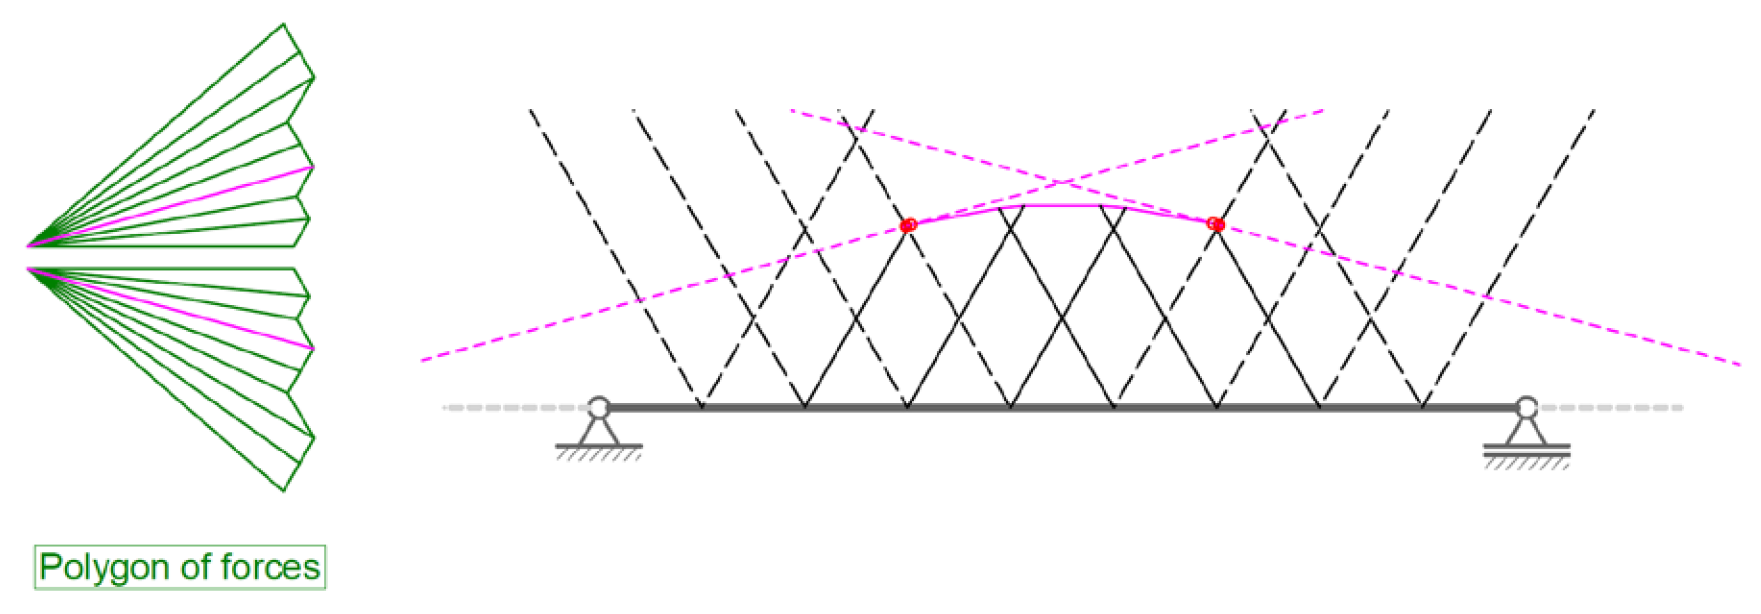
\includegraphics[width=0.9\textwidth]{Pictures/GraphicalThrustLineConstruction.PNG}
    \caption{Graphical construction of the arch shape}
    \label{fig:Cavegn4}
\end{subfigure}
\caption{Optimisation steps \cite{Cavegn}}
\label{fig:Cavegn34}
\end{figure}
It was found, that the obtained arch geometries generally do not correspond to the circular or the parabolic shape. Sometimes they even lie outside of the two traditionally used shapes. By approximating the obtained shape with a quartic function, an analytical expression close to the thrust line was found, deviating by a maximum of 2\% of its height for most arrangements. Further, it was seen that flat angles of inclination lead to thrust lines that are more inclined near the bearing. Ultimately, the impacts under the unilateral live load combinations were used to estimate the generated structure's costs in a comparative study. The Blennerhassett Island Bridge's final design was taken as a reference, and its cost was estimated using unit prices and the quantities specified in the design drawings. The cost of each component in the investigated designs was estimated proportionally to the respective elastic stresses. A flatter hanger inclination reduces the bending moment in the tie and the arch, whereas the maximum hanger forces increased. The estimated costs of the bridge were reduced the most by decreasing inclinations and high initial inclinations. The cost function is thereby minimised by up to 12\%. However, other patterns, such as a constant inclination, performed well if the arch geometry is adapted to the thrust line.


\section{Summary} \label{sec:rev_sum}

The focal point of research on network tied-arch bridges initially lied on the hanger forces. As for short tied-arch bridges, hanger unloading is a critical consideration which initiated the development of this bridge type in the first place.
Along with the increase in popularity of this bridge type in the new millennium, researchers have investigated its manifold aspects. The study of the behaviour under fatigue loading and cable loss put forth demanding challenges. As each of these aspects necessitates a detailed consideration, not one integral design optimisation has been conducted for a network tied-arch bridge. On top of that, the findings of these investigations favour divergent design parameters. The consideration of hanger forces and the behaviour under cable loss favour steep hanger designs, whereas hanger unloading and fatigue are improved by flat arrangements. Further, there are varying boundary conditions, such as the live to dead load ratio, which complicates the formulation of general guidelines. In this challenging environment, it is tempting to combine the objectives into a single score for the results of a parametric study or an objective function for an optimisation method. However, both Teich and Belevicius have exemplified that this approach does not solve the challenges. It only obfuscates the impact of the design variables on the structural behaviour and yields an incomparable score. The lack of knowledge about this bridge type is still too significant. Many aspects have not been investigated sufficiently, which is exemplified by the vague design rules given by the different investigations. The use of advanced optimisation methods cannot overcome this fundamental issue. While focusing on the costs of the structural components helps to put different aspects into perspective, it should be remembered that the cost of labour outweighs material and fabrication costs. Ultimately, Cavegn pointed out, that key design considerations, such as the self-equilibrium stress state and the arch shape, have barely been addressed and require a thorough investigation.


%Further it was pointed out early by \cite{Geissler} that only with a detailed structural model, including accurately modelled knuckles, reliable estimations of the hanger forces can be made.






%\section{Hanger arrangements}
%\paragraph*{Hanger unloading}
%Later, he proposed an arrangement with constant distances between the hanger connection points in the middle of the tie, as shown in \autoref{fig:Tveit}. While the nodes on the arch are spaced equidistantly, the connection points on the tie are constructed with the help of an inclined ellipse and an abscissa and an ordinate depending on the parameters $p_1$ and $p_2$. To determine the points on the tie, linearly spaced vertical lines are drawn to the ellipse. The locations of the nodes on the tie are then determined from the ordinate values of the intersection points.\\
%\begin{figure}[H]
%\centering
%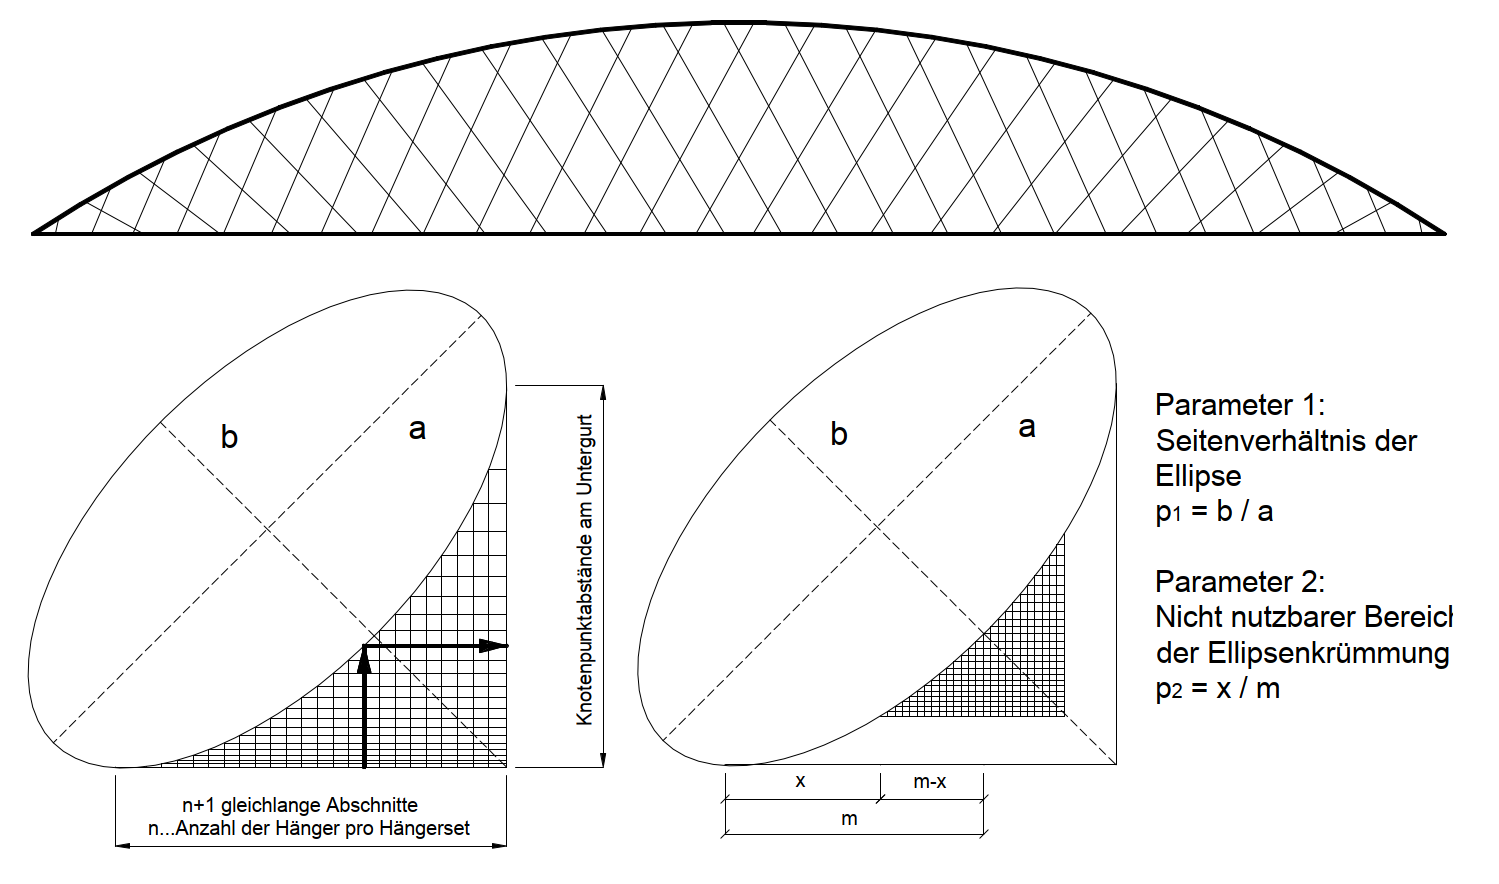
\includegraphics[width=0.7\textwidth]{Pictures/ArrangementTveit.PNG}
%\caption{Arrangement with constant distances in the middle of the tie (adopted from \cite{Teich}).}
%\label{fig:Tveit}
%\end{figure}

%In \cite{Tan} a pedestrian bridge with a sparse hanger arrangement was investigated using an evolutionary optimisation procedure. Each hanger is arranged independently of an overall arrangement. It was found that an arrangement approximately consisting of two separate patterns reduced the internal forces in the arch and the tie the most. Near the knuckles vertical hangers and in the span approximately parallel hangers resulted as shown in \autoref{fig:Tan}.
%\begin{figure}[H]
%\centering
%\begin{subfigure}{0.5\textwidth}
%    \centering
%    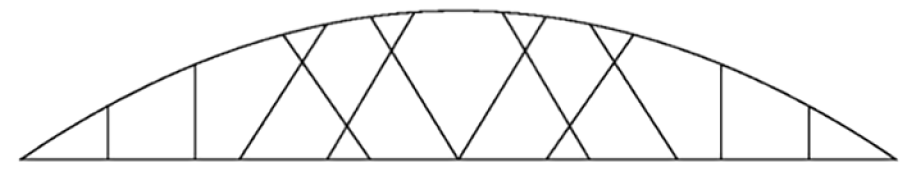
\includegraphics[width=0.9\textwidth]{Pictures/Tan 1.PNG}
%\end{subfigure}%
%\begin{subfigure}{.5\textwidth}
%    \centering
%    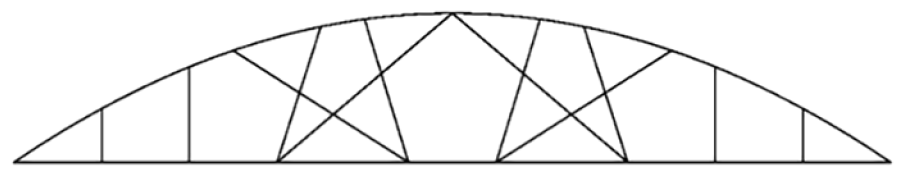
\includegraphics[width=0.9\textwidth]{Pictures/Tan 2.PNG}
%\end{subfigure}
%\caption{Optimal sparse hanger arrangements (adopted from %\cite{Tan}).}
%\label{fig:Tan}
%\end{figure}

%\paragraph*{I don't know}
%In the new millennium, Tveit supervised multiple Master Theses aiming to optimize the design of network tied-arch bridges. In \cite{BrunnSchanack} [nochmals lesen was da genau gemacht wurde]. They developed the radial arrangement aiming to have a pattern which optimally complies with a circular arch. In the radial arrangement, the hangers are equally spaced on the arch and two following hangers cross each other symmetrically to the radius as shown in \autoref{fig:Brunn}. It was the intention, that if the hanger forces are uniform, the thrust line also approximately corresponds to a circle, resulting in an efficient use of the arch. In the literature, this arrangement is either described by the angle $\alpha$ between the arch and the hanger or by the angle $\beta$ between the hangers and the radius at the first intersection point.

%\begin{figure}[H]
%\centering
%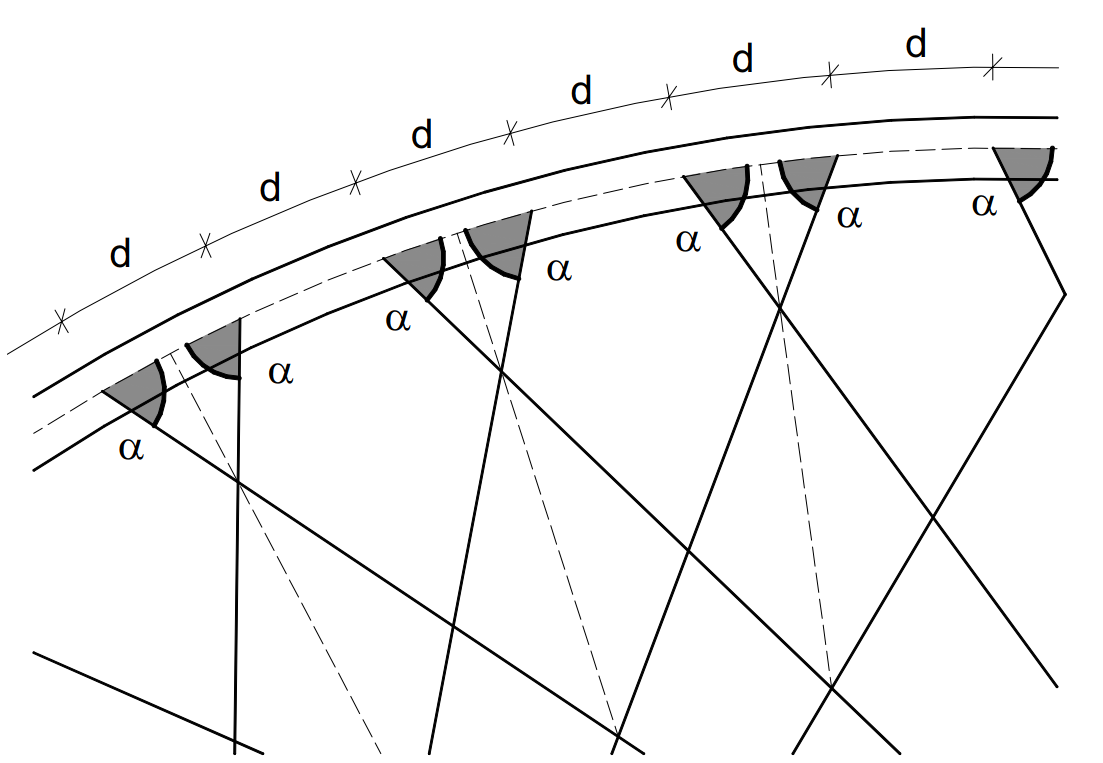
\includegraphics[width=0.4\textwidth]{Pictures/RadialArrangement.PNG}
%\caption{Radial hanger arrangement (adopted from \cite{BrunnSchanack2}).}
%\label{fig:Brunn}
%\end{figure}

%Both of the authors continued their work in the field of network tied-arch bridges and conclude their findings in \cite{BrunnSchanack2}. Besides the bending moments and the maximum hanger forces, also the variation of hanger forces, which are relevant for fatigue, and the elastic embedding of the arch is focused on. These objectives are evaluated manually/arbitrarily. In a comparison of the different hanger patterns, it is concluded that parallel hangers are disadvantageous concerning the bending moments in the arch as the hanger forces vary strongly. Angles of inclination between $55\degree$ and $60\degree$ give the best results. For the constant change of inclination arrangement the middle hanger was recommended to be inclined in the similar range from $56\degree$ to $60\degree$. Further, the change of inclination between two following hangers should lead to an inclination of up to $80\degree$ in the steepest hangers. The radial arrangement was considered optimal, especially for the small corresponding variation of maximum hanger forces and uniform embedding of the arch. The angle between the hangers and the arch are recommended to be between $55\degree$ and $60\degree$. Interestingly, the optimal solutions for each hanger arrangement feature a middle hanger with an inclination of $55\degree$ to $60\degree$. Further, it is recommended that the hanger spacing on the arch lies between \SI{2.5}{m} and \SI{4}{m}.

